\documentclass{beamer}
%\usepackage[utf8]{inputenc}
%\usepackage{graphicx}
%usepackage {mathtools}
%\usepackage{utopia} %font utopia imported
\usetheme{CambridgeUS}
%\usecolortheme{default}
\usepackage{minted}
%\usefonttheme{professionalfonts}
%\usepackage{natbib}
%\usepackage{hyperref}
\usepackage{colortbl}
\usepackage{pifont} % Custom bullets
%------------------------------------------------------------
% set colors
\definecolor{greyColor}{RGB}{242,242,245} % grey
\definecolor{greenColor}{RGB}{51,112,98} % green
\definecolor{yellowColor}{RGB}{246,202,84} % yellow
\definecolor{blackColor}{RGB}{84,84,84} % yellow
%------------------------------------------------------------
\setbeamercolor*{palette primary}{bg=yellowColor}
\setbeamercolor*{palette secondary}{bg=greyColor}
\setbeamercolor*{palette tertiary}{bg=greenColor, fg = white}
\setbeamercolor*{titlelike}{fg=greyColor}
\setbeamercolor*{title}{bg=greenColor, fg = white}
\setbeamercolor*{item}{fg=blackColor}
\setbeamercolor*{caption}{fg=greenColor}
\setbeamercolor{frametitle}{fg=black,bg=greyColor}

% customize the caption
\setbeamerfont{caption}{size=\footnotesize}
\setbeamercolor{caption}{fg=blackColor}
\setbeamercolor{caption name}{fg=greenColor}

% https://latex-beamer.com/tutorials/blocks/
\setbeamertemplate{blocks}[rounded][shadow=true]
\setbeamercolor{block title}{bg=greenColor, fg=white}
\setbeamercolor{block body}{bg=greyColor, fg=blackColor}

% see https://pygments.org/styles/
\usemintedstyle{solarized-light}
% [bgcolor=greyColor,linenos, breaklines,frame=leftline, numbersep=1pt,mathescape]
\setminted[shell]{bgcolor=greyColor, breaklines, numbersep=1pt,mathescape, fontsize=\footnotesize}
\setminted[rust]{bgcolor=greyColor,linenos, breaklines,frame=leftline, numbersep=1pt,mathescape, fontsize=\footnotesize}
\setminted[toml]{bgcolor=greyColor,linenos, breaklines,frame=leftline, numbersep=1pt,mathescape, fontsize=\footnotesize}
%------------------------------------------------------------
\title[Rust-Lang]{Rust Programming Language}
\author[Yumcoder]{Yumcoder}

\institute[UoT]{University of Toronto}
\date[{\today} ]
{\today}
%------------------------------------------------------------
%This block of commands puts the table of contents at the 
%beginning of each section and highlights the current section:
%\AtBeginSection[]
%{
	%  \begin{frame}
		%    \frametitle{Contents}
		%    \tableofcontents[currentsection]
		%  \end{frame}
	%}
\AtBeginSection[]{
	\begin{frame}
		\vfill
		\centering
		\begin{beamercolorbox}[sep=8pt,center,shadow=true,rounded=true]{title}
			\usebeamerfont{title}\insertsectionhead\par%
		\end{beamercolorbox}
		\vfill
	\end{frame}
}
%------------------------------------------------------------

\begin{document}
	
	%The next statement creates the title page.
	\frame{\titlepage}
	\begin{frame}
		\frametitle{Contents}
		\mbox{
			\linespread{2.3}
			\tiny
			\begin{columns}
				\column{0.5\textwidth}
				\tableofcontents[sections = 1-10]
				\column{0.5\textwidth}
				\tableofcontents[sections = 11-20]
		\end{columns}
	}
	\end{frame}
	%------------------------------------------------------------
	\section{Introduction}
	\begin{frame}[fragile]
		\frametitle{Installing rustup on Linux or macOS}
		If you’re using Linux or macOS, open a terminal and enter the following command:
		
		\inputminted{shell}{./code/install.shell}
		If the install is successful, the following line will appear:
		\begin{minted}[linenos=false, breaklines,frame=none]{shell}
			Rust is installed now. Great!
		\end{minted}
		To check whether you have Rust installed correctly, open a shell and enter this line:
		\inputminted{shell}{./code/install-check.shell}
	\end{frame}
	
	\begin{frame}[fragile]
		\frametitle{Updating, Uninstalling and Local Documentation}
		Once Rust is installed via rustup, when a new version of Rust is released, updating to the latest version is easy. From your shell, run the following update script:
		
		\inputminted{shell}{./code/install-update.shell}
		
		To uninstall Rust and rustup, run the following uninstall script from your shell:
		\inputminted{shell}{./code/install-uninstall.shell}
		
		The installation of Rust also includes a local copy of the documentation, so you can read it offline. Run \mintinline{shell}{rustup doc}  to open the local documentation in your browser.
	\end{frame}
	
	\begin{frame}[fragile]
		\frametitle{Hello, World!}
		Open a terminal and enter the following commands:
		
		\inputminted[linenos, breaklines,frame=leftline, numbersep=1pt]{shell}{./code/hello-world.shell}
		
		Make a new source file and save it as main.rs:
		\inputminted{rust}{./code/hello-world-main.rs}
		
		Compile and run the file:
		\inputminted{shell}{./code/hello-world-compile.shell}
	\end{frame}
	
	\begin{frame}[fragile]
		\frametitle{Cargo}
		\begin{itemize}
			\item Cargo is \textbf{Rust’s build system and package manager}. 
			\item Most \textbf{Rustaceans} use this tool to manage their Rust projects because Cargo handles a lot of tasks for you, such as building your code, downloading the libraries your code depends on, and building those libraries. 
			\begin{itemize}
				\item[\ding{43}] \textbf{Rustaceans} are people who use Rust, contribute to Rust, or are interested in the development of Rust.
			\end{itemize}
			\item  Cargo comes installed with Rust if you used the official installer.
			\begin{itemize}
				\item[] \inputminted{shell}{./code/cargo.shell}
			\end{itemize}
		\end{itemize}
	\end{frame}
	
	\begin{frame}[fragile]
		\frametitle{Hello, Cargo!}
		Creating a Project with Cargo:
		\inputminted{shell}{./code/hello-cargo.shell}
		
		\begin{figure}
			\centering
			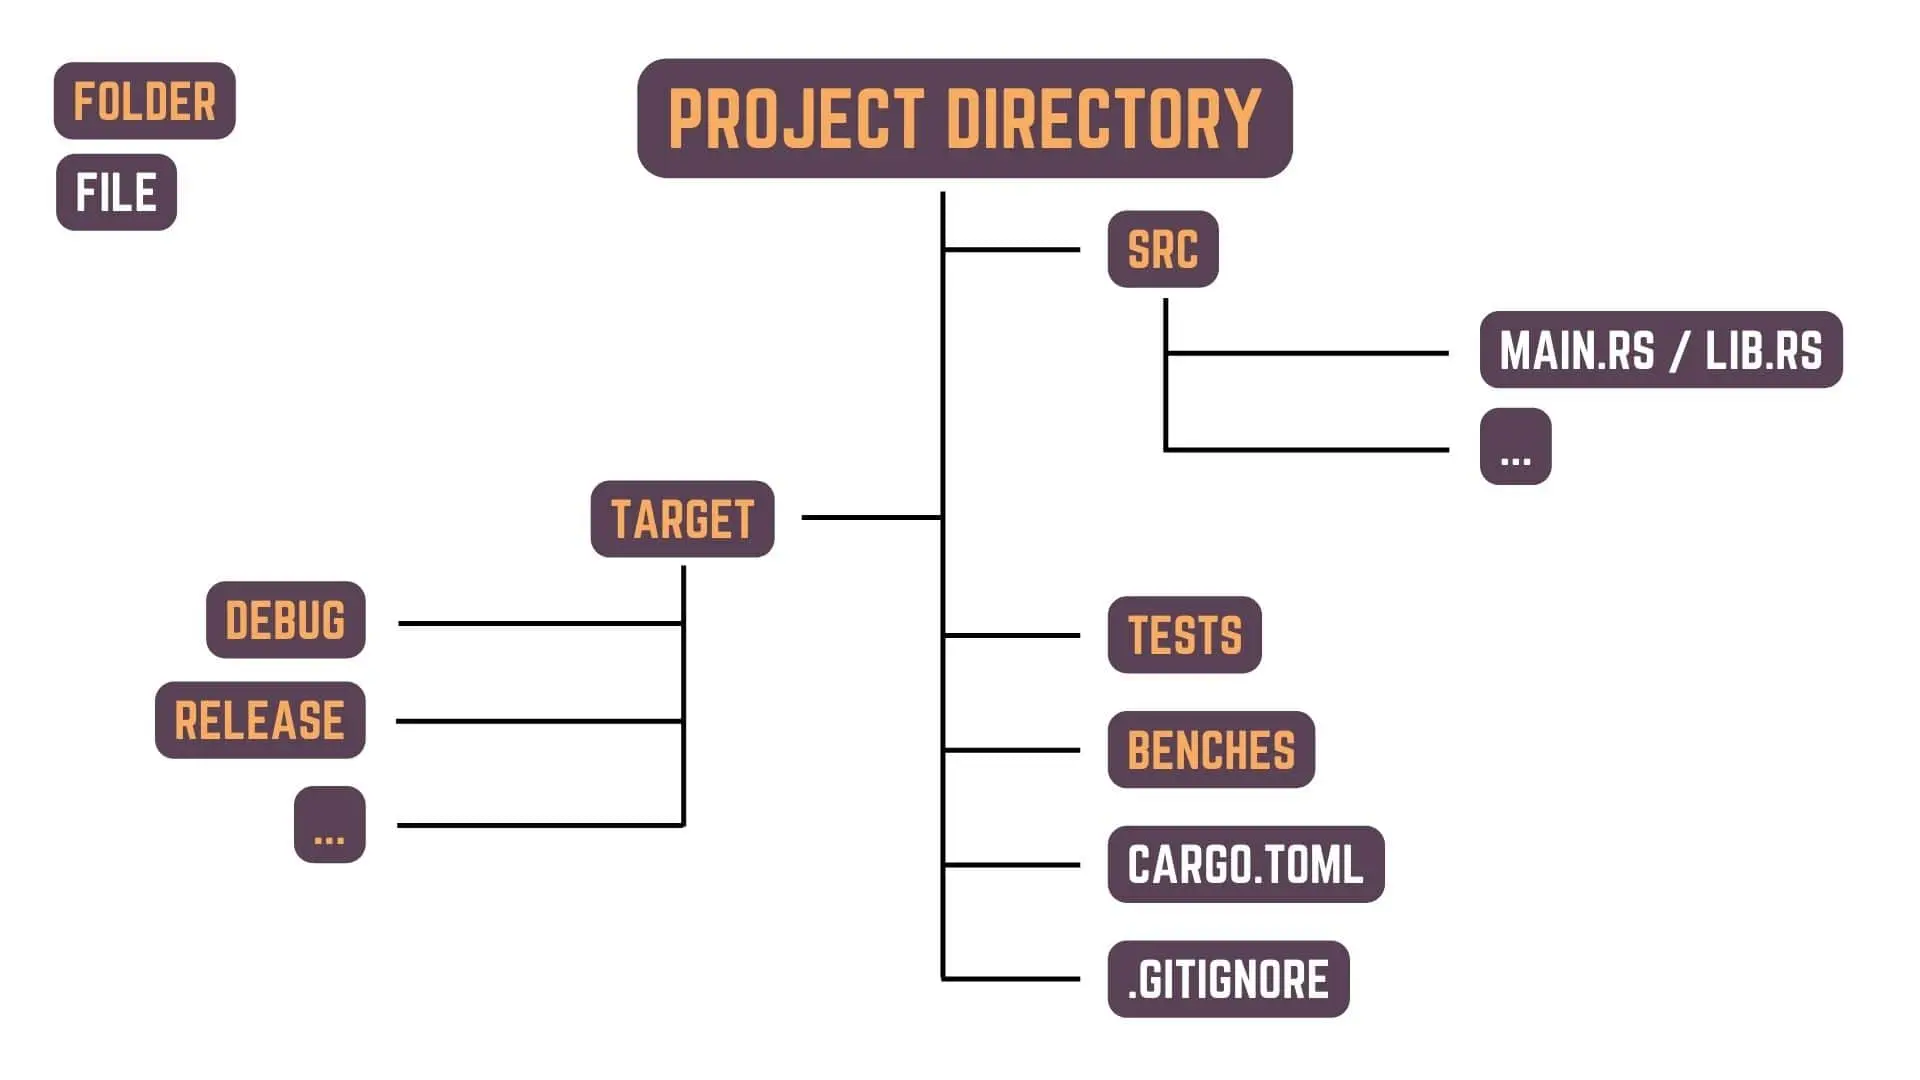
\includegraphics[width=0.65\textwidth]{./img/rust-project-folder-structure.png}
			\caption{Folder structure for projects in rust programming language.}
			\label{fig:folderRustLang}
		\end{figure}
	\end{frame}
	
	\begin{frame}[fragile]
		\frametitle{Cargo.toml}
		This file is in the \textbf{TOML} (Tom’s Obvious, Minimal Language) format, which is \textbf{Cargo’s configuration} format.
		
		\inputminted{toml}{./code/cargo.toml}
	\end{frame}
	
	\begin{frame}[fragile]
		\frametitle{Building and Running a Cargo Project}
		Now open src/main.rs and take a look:
		\inputminted{rust}{./code/hello-world-main.rs}
		
		Build your project by entering the following command:
		
		\inputminted{shell}{./code/hello-world-build.shell}
		
		\begin{itemize}
			\item Use \mintinline{shell}{cargo run} to compile and then run (all in one command).
			\item When your project is finally ready for release, you can use \mintinline{shell}{cargo build --release} to compile it with optimizations (create an executable in target/release instead of target/debug). 
		\end{itemize}
	\end{frame}
	
	\section{Common Programming Concepts}
	
	\begin{frame}{Variables and Mutability}
		\begin{itemize}
			\item by default variables are \textbf{immutable}. 
			\item This is one of many \textbf{\href{https://en.wikipedia.org/wiki/Nudge_theory}{\underline{nudges}} Rust}   gives you to write your code in a way that takes advantage of the \textbf{safety and easy concurrency }that Rust offers. 
			\begin{itemize}
				\item However, you still have the option to make your variables \textbf{mutable}. 
			\end{itemize}
		\end{itemize}
	\end{frame}
	
	\begin{frame}[fragile]
		\frametitle{Immutable variables}
		When a variable is immutable, \textit{once a value is bound to a name, you can’t change that value.}
		
		\inputminted{rust}{./code/immutable-variable.rs}
	\end{frame}
	
	\begin{frame}[fragile]
		\frametitle{Immutable variables (2)}
		You should receive an error message, as shown in this output:
		
		\inputminted{shell}{./code/immutable-variable.shell}
	\end{frame}
	
	\begin{frame}[fragile]
		\frametitle{Mutable variables}
		Although variables are immutable by default, you can make them mutable by adding \mintinline{rust}{mut} in front of the variable name.
		
		\inputminted{rust}{./code/mutable-variable.rs}
	\end{frame}
	
	\begin{frame}[fragile]
		\frametitle{Mutable variables (2)}
		\inputminted{shell}{./code/mutable-variable.shell}
	\end{frame}
	
	\begin{frame}[fragile]
		\frametitle{Constants}
		Rust’s naming convention for constants is to use \textit{all uppercase with underscores between words}.
		\inputminted[linenos=false, frame=none]{rust}{./code/const.rs}
		Like immutable variables, constants are values that are bound to a name and are not allowed to change, but there are a few differences between constants and variables.
		
		\begin{itemize}
			\item you aren’t allowed to use \mintinline{rust}{mut} with constants. Constants aren’t just immutable by default—\textbf{they’re always immutable}. You declare constants using the const keyword instead of the let keyword, and \textbf{the type of the value must be annotated}.
			
			\item 		constants may be set only to a constant expression, \textbf{not the result of a value that could only be computed at runtime}.
		\end{itemize}
	\end{frame}
	
	\begin{frame}[fragile]
		\frametitle{Shadowings}
		Rustaceans say that the first variable is shadowed by the second, which means that the second variable is what the compiler will see when you use the name of the variable.  We can shadow a variable by using the same variable’s name and repeating the use of the \mintinline{rust}{let} keyword as follows
		
		\inputminted{rust}{./code/shadowing.rs}
	\end{frame}
	
	\begin{frame}[fragile]
		\frametitle{Shadowing (2)}
		\inputminted{shell}{./code/shadowing.shell}
	\end{frame}
	
	\begin{frame}[fragile]
		\frametitle{Shadowing vs Mutable variables}
		
		We’re effectively creating a new variable when we use the let keyword again, we can change the type of the value but reuse the same name.
		
		\begin{columns}
			\column{0.5\textwidth}
			\inputminted{rust}{./code/shadowing-vs-mutable-var1.rs}
			The first spaces variable is a string type and the second spaces variable is a number type. 
			\column{0.5\textwidth}
			\inputminted{rust}{./code/shadowing-vs-mutable-var2.rs}
			we’ll get a \textbf{compile-time error}: mismatched types, expected `\&str`, found `usize`.
		\end{columns}
	\end{frame}
	
	\begin{frame}[fragile]
		\frametitle{Data Types}
		\begin{columns}
			\column{0.5\textwidth}
			Data type subsets: 
			\begin{itemize}
				\item Scalar
				\begin{itemize}
					\item Integers
					\item Floating-point numbers
					\item Booleans
					\item Characters
				\end{itemize}
				\item Compound
				\begin{itemize}
					\item Tuples 
					\item Arrays
				\end{itemize}
			\end{itemize}
			\column{0.5\textwidth}
			\inputminted{rust}{./code/data-types.rs}
		\end{columns}
		
		\begin{block}{Statically typed language}
			Keep in mind that Rust is a statically typed language, which means that \textbf{it must know the types of all variables at compile time}. 
		\end{block}
		
		The compiler can usually \textbf{infer} what type we want to use based on the value and how we use it (example: \mintinline{rust}{let x = 2.0; // f64}).
		
	\end{frame}
	
	\begin{frame}[fragile]
		\frametitle{Integer Types}
		\begin{itemize}
			\item An integer is a number without a fractional component.
			\item This type declaration indicates that the value it’s associated with should be an unsigned integer (signed integer types start with \textbf{i}, instead of \textbf{u}) that takes up 32 bits of space.
		\end{itemize}
		
		\begin{table}
			\begin{tabular}{|c|c|c|}
				\hline
				\rowcolor{greyColor}
				Length & Signed & Unsigned \\
				\hline
				8-bit & i8 & u8 \\
				16-bit & i16 & u16 \\
				32-bit & i32 & u32 \\
				64-bit & i64 & u64 \\
				128-bit & i128 & u128 \\
				arch\footnote{the isize and usize types depend on the architecture: 64 bits if you’re on a 64-bit architecture and 32 bits if you’re on a 32-bit architecture.} & isize & usize \\
				\hline
			\end{tabular}
		\end{table}
		
	\end{frame}
	
	\begin{frame}[fragile]
		\frametitle{Integer literals}
		\begin{itemize}
			\item A number literal is a type suffix, such as \mintinline{rust}{57u8}, to designate the type
			\item Number literals can also use \mintinline{rust}{_} as a visual separator to make the number easier to read, such as  \mintinline{rust}{1_000} , which will have the same value as if you had specified \mintinline{rust}{1000}
		\end{itemize}
		\begin{table}
			\begin{tabular}{|c|c|}
				\hline
				\rowcolor{greyColor}
				Number literals	& Example \\
				\hline
				Decimal & \mintinline{rust}{let x = 98_222} \\
				Hex & \mintinline{rust}{let x = 0xff} \\
				Octal & \mintinline{rust}{let x = 0o77} \\
				Binary & \mintinline{rust}{let x = 0b1111_0000} \\
				Byte (u8 only) & \mintinline{rust}{let x = b'A'} \\
				\hline
			\end{tabular}
		\end{table}
	\end{frame}
	
	\begin{frame}[fragile]
		\frametitle{Integer Overflow}
		\begin{itemize}
			\item Let’s say you have a variable of type u8 that can hold values between 0 and 255. 
			\item 		If you try to change the variable to a value outside of that range, such as 256, integer overflow will occur, which can result in one of two behaviors:
			\begin{itemize}
				\item When you’re compiling in \textbf{debug mode}, Rust includes checks for integer overflow that cause your program to panic at runtime if this behavior occurs.
				\item 		When you’re compiling in \textbf{release mode} with the --release flag, Rust does not include checks for integer overflow that cause panics (In the case of a u8, the value 256 becomes 0, the value 257 becomes 1, and so on).
			\end{itemize}
		\end{itemize}
	\end{frame}
	
	\begin{frame}[fragile]
		\frametitle{Floating-Point Types}
		\begin{itemize}
			
			\item Rust’s floating-point types are f32 (32 bits) and f64(64 bits), see (\href{https://en.wikipedia.org/wiki/IEEE_754}{\textsc{IEEE-754 standard}}).
			
			\item The default type is f64 because on modern CPUs it’s roughly the same speed as f32 but is capable of more precision. 
			\item All floating-point types are signed.
		\end{itemize}
		\begin{columns}
			\column{0.5\textwidth}
			\inputminted{rust}{./code/floating-types.rs}
			\column{0.5\textwidth}
			\inputminted{rust}{./code/IEEE-754.rs}
		\end{columns}
	\end{frame}
	
	\begin{frame}[fragile]
		\frametitle{Numeric Operations}
			\inputminted{rust}{./code/numeric-operations.rs}
	\end{frame}

	\begin{frame}[fragile]
		\frametitle{Boolean Types}
		Booleans are one byte in size.
		
		\inputminted{rust}{./code/bool-types.rs}
	\end{frame}


	\begin{frame}[fragile]
		\frametitle{Character Types}
		\begin{itemize}
			\item Note that we specify char literals with \textbf{single quotes}, as opposed to string literals, which use double quotes. 
			\item Rust’s char type is four bytes in size and represents a Unicode Scalar Value, which means it can represent a lot more than just ASCII.
		\end{itemize}
		
		\inputminted{rust}{./code/char-types.rs}
	\end{frame}


	\section{Understanding Ownership}  
	\section{Using Structs to Structure Related Data}  
	\section{Enums and Pattern Matching}  
	\section{Managing Projects with Packages, Crates, and Modules}
	\section{Common Collections}  
	\section{Error Handling}  
	\section{Generic Types, Traits, and Lifetimes}  
	\section{Writing Automated Tests}  
	\section{An I/O Project: Building a Command Line Program}  
	\section{Functional Language Features: Iterators and Closures}  
	\section{More About Cargo and Crates.io}  
	\section{Smart Pointers}  
	\section{Fearless Concurrency}  
	\section{Object-Oriented Programming Features of Rust}  
	\section{Patterns and Matching}  
	\section{Advanced Features}  
	\section{Multithread Web Server}  
	\section{Tokio}  
	
	\section*{Acknowledgement}  
	\begin{frame}
		\Huge{\centerline{Thank you!}}
	\end{frame}
	
\end{document}

\begin{comment}
	\begin{frame}[fragile]
		\frametitle{title}
	\end{frame}
\end{comment}


